\documentclass{beamer}

\usepackage{graphicx}
\usepackage{enumerate}
\usepackage{framed}
\usepackage{amsmath}

\begin{document}
	\begin{frame}
		\Huge
		\[\mbox{Linkage of Health Information} \] \[\mbox{in the Irish Health System:} \] \[\mbox{Challenges \& Solutions} \]
		\bigskip
		\Large
		\[\mbox{Kevin Patrick O'Brien} \]
	\end{frame}
%============================================ %
\begin{frame}
	\begin{figure}
		\centering
		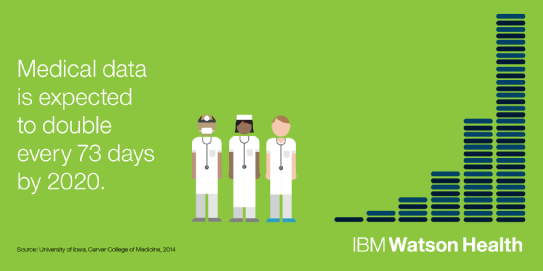
\includegraphics[width=0.99\linewidth]{medicaldata}
		
	\end{figure}
	\textbf{Medical Data is expected to double every 73 days by 2020}\\
	(A lot of clinical measurements)
	
\end{frame}	

		%=========================================%
		
		\begin{frame}
			\Large
			\textbf{Hospital Data}
			
			\begin{itemize}
				\item Hospital In-Patient Enquiry (HIPE) system.
				\item Computer based system for administrative health data.
				\item Systematically collecting data since early 90s.
				\item Formerly part of ESRI, now part of HSE.
			\end{itemize} 


		\end{frame}
\begin{frame}
	\begin{figure}
\centering
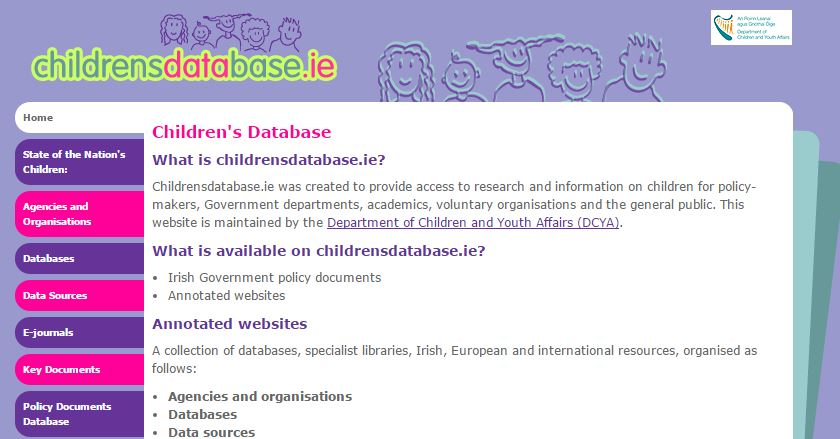
\includegraphics[width=1.19\linewidth]{childrensdatabase}

\end{figure}

\end{frame}

		%=========================================%
	\begin{frame}
		
		\begin{figure}
\centering

\includegraphics[width=1.19\linewidth]{irishprimarycarenetwork}


\end{figure}

	\end{frame}	
		\begin{frame}
			\Large
			\textbf{Pooling Data}
			\begin{itemize}
				\item Health Boards and GPs need to be brought on board.
			%	\item Need to get stakeholders to ``Buy In".
				\item Communicate benefits of sharing and pooling data for syudying population health.
				\item Negative cases used in contrast with positive cases.
				\item Privacy Issues, Statistical Disclosure Control.
			\end{itemize}
		\end{frame}


\begin{frame}
\begin{figure}
\centering
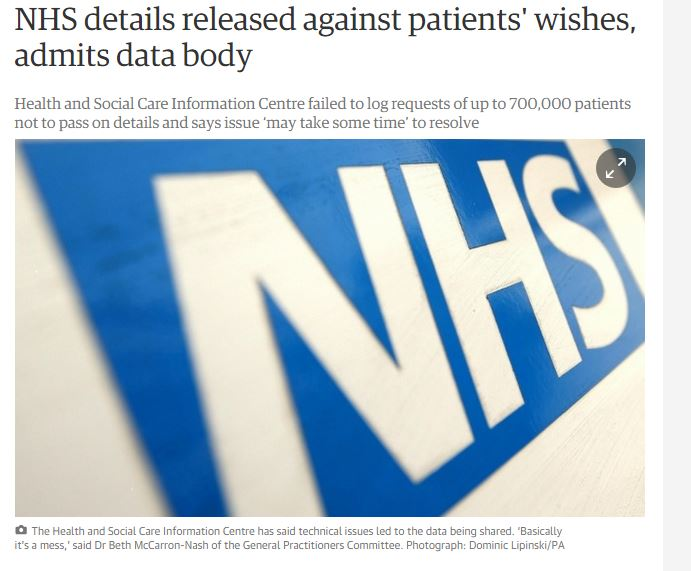
\includegraphics[width=0.99\linewidth]{NHSdata}
\end{figure}

\end{frame}	
	%========================================%
		\begin{frame}
			\Large
			\textbf{Unique Idenifiers}
			\begin{itemize}
				\item In Database Science - Primary Keys
				\item Which Kevin O'Brien are we talking about?
				\item PPS number.
				\item Which Crescent Court are we talking about? (Later)
			\end{itemize}
		\end{frame}


%============================================ %
\begin{frame}
\frametitle{Personal Identifers}
\Large
\begin{itemize}
	\item \textit{Personnumber}
	\item Unique Identifier for all residents of Sweden
\end{itemize}
\begin{figure}
\centering
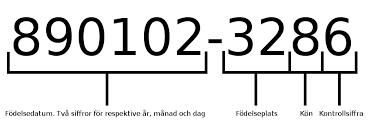
\includegraphics[width=0.9\linewidth]{personnummerSweden}
%\caption{Source: Wikipedia.com}
\end{figure}
{
\normalsize \textit{Wikipedia.com}
}
\end{frame}
%============================================= %
\begin{frame}
	\Large
	\textbf{Unique Identifiers for Medical Records}\bigskip
	\begin{itemize}
		\item Various Regional Healthboards.
		\item Public and Private hospitals.
		\item Can't assume same operating procedures for medical data.
		\item Is the available data machine readable? 
		\item (Open Data 5 star system).
		\item Manual Data Cleaning : deleting meta data.
	\end{itemize}
\end{frame}
%============================================= %	
		\begin{frame}
			\Large
		\textbf{Probabilistic Record Linkage}
\begin{quote}
	Probabilistic record linkage.... takes a different approach to the record linkage problem by taking into account a wider range of potential identifiers, computing weights for each identifier based on its estimated ability to correctly identify a match or a non-match, and using these weights to calculate the probability that two given records refer to the same entity. (\textit{Wikipedia})
\end{quote}
		\end{frame}
	%=============================================== %
\begin{frame}
	\Large
	\textbf{Record Linkage - R Packages}
	\begin{figure}
\centering
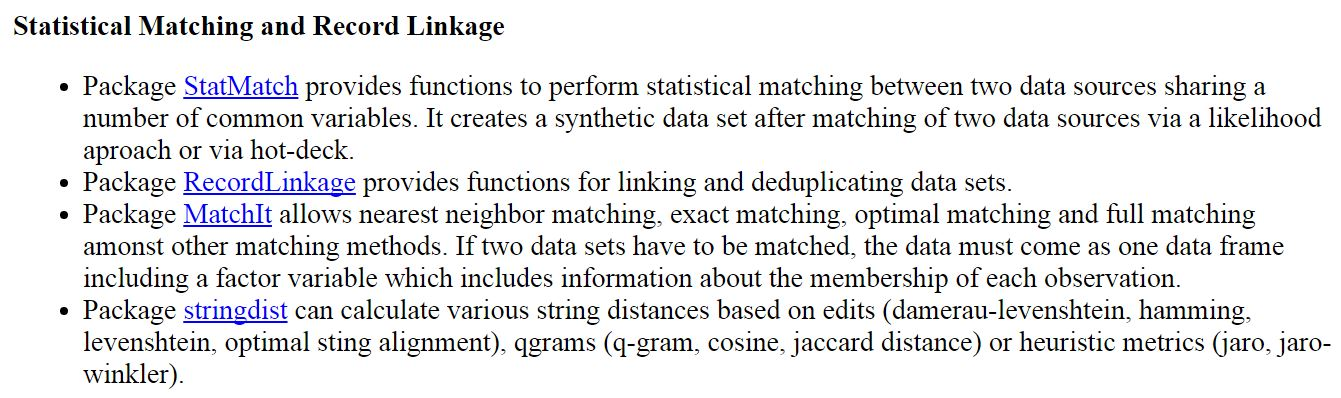
\includegraphics[width=1.4\linewidth]{Rpackages}

\end{figure}

	
\end{frame}
	%=============================================== %
	\begin{frame}
		\Large
		\textbf{Record Linkage - R Packages}
		\begin{figure}
			\centering
			
\includegraphics[width=1.1\linewidth]{Rpackages2}
			
		\end{figure}
		
		
	\end{frame}
%============================================== %
\begin{frame}
	\frametitle{Spatial Analyses}
	\begin{figure}
		\centering
		
		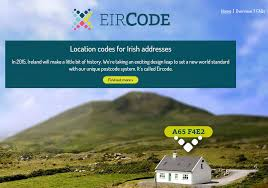
\includegraphics[width=0.5\linewidth]{Eircode}
		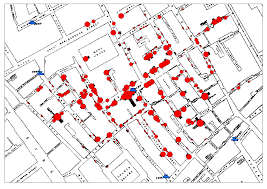
\includegraphics[width=0.5\linewidth]{johnsnowmap}
		
	\end{figure}
{
	\normalsize Source: \textit{eircode.ie} and \textit{Wikipedia.com}
}	
\end{frame}
%============================================ %
\begin{frame}
	\Large
	\textbf{Unique Location Identifiers}
	
	\begin{itemize}
		\item Population Health Analyses.
		\item John Snow's Cholera Map.
		\item How would we do something like that now?
		\item Eircode (proprietary system).
		\item Can locations be identified as ``near" based on codes?
	\end{itemize}
\end{frame}


\end{document}
